\section{CTCLVariable  Class Reference}
\label{classCTCLVariable}\index{CTCLVariable@{CTCLVariable}}
{\tt \#include $<$TCLVariable.h$>$}

Inheritance diagram for CTCLVariable::\begin{figure}[H]
\begin{center}
\leavevmode
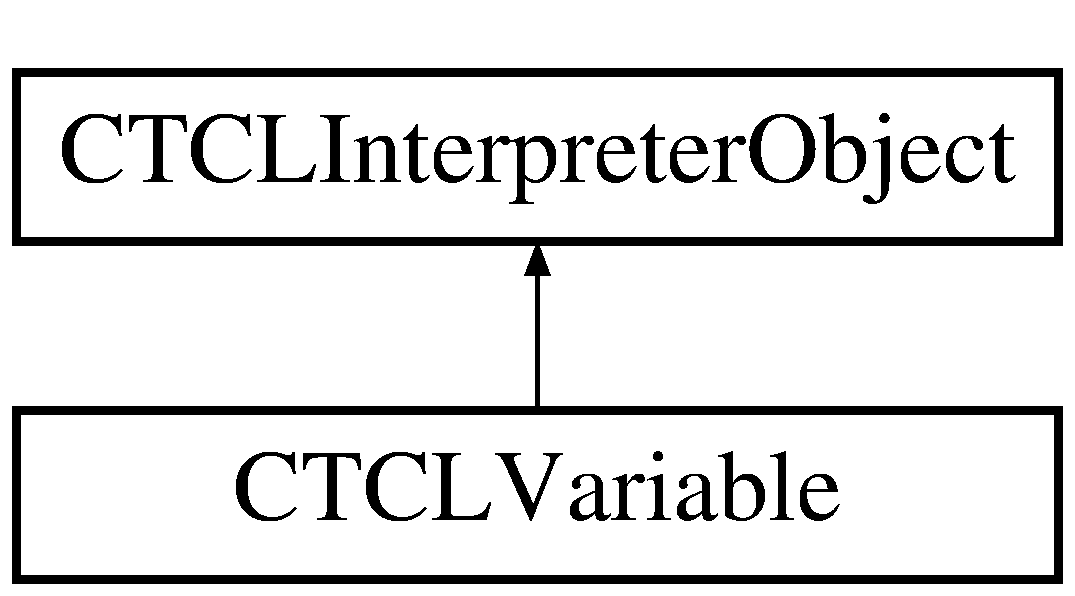
\includegraphics[height=2cm]{classCTCLVariable}
\end{center}
\end{figure}
\subsection*{Public Methods}
\begin{CompactItemize}
\item 
{\bf CTCLVariable} (std::string am\_\-s\-Variable, {\bf Bool\_\-t} am\_\-f\-Tracing)
\item 
{\bf CTCLVariable} ({\bf CTCLInterpreter} $\ast$p\-Interp, std::string am\_\-s\-Variable, {\bf Bool\_\-t} am\_\-f\-Tracing)
\item 
{\bf $\sim$CTCLVariable} ()
\item 
{\bf CTCLVariable} (const CTCLVariable \&a\-CTCLVariable)
\item 
CTCLVariable \& {\bf operator=} (const CTCLVariable \&a\-CTCLVariable)
\item 
int {\bf operator==} (const CTCLVariable \&a\-CTCLVariable) const
\item 
std::string {\bf get\-Variable\-Name} () const
\item 
{\bf Bool\_\-t} {\bf Is\-Tracing} () const
\item 
void {\bf set\-Variable\-Name} (const std::string am\_\-s\-Variable)
\item 
virtual char $\ast$ {\bf operator()} (char $\ast$p\-Name, char $\ast$p\-Subscript, int Flags)
\item 
virtual const char $\ast$ {\bf Set} (const char $\ast$p\-Value, int flags=TCL\_\-LEAVE\_\-ERR\_\-MSG$|$TCL\_\-GLOBAL\_\-ONLY)
\item 
virtual const char $\ast$ {\bf Set} (const char $\ast$p\-Subscript, char $\ast$p\-Value, int flags=TCL\_\-LEAVE\_\-ERR\_\-MSG$|$TCL\_\-GLOBAL\_\-ONLY)
\item 
virtual const char $\ast$ {\bf Get} (int flags=TCL\_\-LEAVE\_\-ERR\_\-MSG$|$TCL\_\-GLOBAL\_\-ONLY, char $\ast$p\-Index=0)
\item 
int {\bf Link} (void $\ast$p\-Variable, int Type)
\item 
void {\bf Unlink} ()
\item 
int {\bf Trace} (int flags=TCL\_\-TRACE\_\-READS$|$TCL\_\-TRACE\_\-WRITES$|$TCL\_\-TRACE\_\-UNSETS, char $\ast$p\-Index=(char $\ast$) {\bf kp\-NULL})
\item 
void {\bf Un\-Trace} ()
\item 
void {\bf Update} ()
\end{CompactItemize}
\subsection*{Static Public Methods}
\begin{CompactItemize}
\item 
char $\ast$ {\bf Trace\-Relay} (Client\-Data p\-Object, Tcl\_\-Interp $\ast$p\-Interpreter, char $\ast$p\-Name, char $\ast$p\-Index, int flags)
\end{CompactItemize}
\subsection*{Protected Methods}
\begin{CompactItemize}
\item 
void {\bf set\-Tracing} ({\bf Bool\_\-t} am\_\-f\-Tracing)
\item 
void {\bf Do\-Assign} (const CTCLVariable \&r\-Rhs)
\end{CompactItemize}
\subsection*{Private Attributes}
\begin{CompactItemize}
\item 
std::string {\bf m\_\-s\-Variable}
\item 
{\bf Bool\_\-t} {\bf m\_\-f\-Tracing}
\item 
{\bf Int\_\-t} {\bf m\_\-n\-Trace\-Flags}
\item 
std::string {\bf m\_\-s\-Trace\-Index}
\end{CompactItemize}


\subsection{Constructor \& Destructor Documentation}
\index{CTCLVariable@{CTCLVariable}!CTCLVariable@{CTCLVariable}}
\index{CTCLVariable@{CTCLVariable}!CTCLVariable@{CTCLVariable}}
\subsubsection{\setlength{\rightskip}{0pt plus 5cm}CTCLVariable::CTCLVariable (std::string {\em am\_\-s\-Variable}, {\bf Bool\_\-t} {\em am\_\-f\-Tracing})\hspace{0.3cm}{\tt  [inline]}}\label{classCTCLVariable_a0}




Definition at line 320 of file TCLVariable.h.

References Bool\_\-t, m\_\-f\-Tracing, and m\_\-s\-Variable.\index{CTCLVariable@{CTCLVariable}!CTCLVariable@{CTCLVariable}}
\index{CTCLVariable@{CTCLVariable}!CTCLVariable@{CTCLVariable}}
\subsubsection{\setlength{\rightskip}{0pt plus 5cm}CTCLVariable::CTCLVariable ({\bf CTCLInterpreter} $\ast$ {\em p\-Interp}, std::string {\em am\_\-s\-Variable}, {\bf Bool\_\-t} {\em am\_\-f\-Tracing})\hspace{0.3cm}{\tt  [inline]}}\label{classCTCLVariable_a1}




Definition at line 325 of file TCLVariable.h.

References Bool\_\-t, m\_\-f\-Tracing, and m\_\-s\-Variable.\index{CTCLVariable@{CTCLVariable}!~CTCLVariable@{$\sim$CTCLVariable}}
\index{~CTCLVariable@{$\sim$CTCLVariable}!CTCLVariable@{CTCLVariable}}
\subsubsection{\setlength{\rightskip}{0pt plus 5cm}CTCLVariable::$\sim$CTCLVariable ()}\label{classCTCLVariable_a2}




Definition at line 312 of file TCLVariable.cpp.

References m\_\-s\-Variable, and Un\-Trace().\index{CTCLVariable@{CTCLVariable}!CTCLVariable@{CTCLVariable}}
\index{CTCLVariable@{CTCLVariable}!CTCLVariable@{CTCLVariable}}
\subsubsection{\setlength{\rightskip}{0pt plus 5cm}CTCLVariable::CTCLVariable (const CTCLVariable \& {\em a\-CTCLVariable})\hspace{0.3cm}{\tt  [inline]}}\label{classCTCLVariable_a3}




Definition at line 334 of file TCLVariable.h.

References Do\-Assign(), m\_\-f\-Tracing, and m\_\-s\-Variable.

\subsection{Member Function Documentation}
\index{CTCLVariable@{CTCLVariable}!DoAssign@{DoAssign}}
\index{DoAssign@{DoAssign}!CTCLVariable@{CTCLVariable}}
\subsubsection{\setlength{\rightskip}{0pt plus 5cm}void CTCLVariable::Do\-Assign (const CTCLVariable \& {\em r\-Rhs})\hspace{0.3cm}{\tt  [protected]}}\label{classCTCLVariable_b1}




Definition at line 618 of file TCLVariable.cpp.

References m\_\-f\-Tracing, m\_\-n\-Trace\-Flags, m\_\-s\-Trace\-Index, m\_\-s\-Variable, Trace(), and Un\-Trace().

Referenced by CTCLVariable(), and operator=().\index{CTCLVariable@{CTCLVariable}!Get@{Get}}
\index{Get@{Get}!CTCLVariable@{CTCLVariable}}
\subsubsection{\setlength{\rightskip}{0pt plus 5cm}const char $\ast$ CTCLVariable::Get (int {\em flags} = TCL\_\-LEAVE\_\-ERR\_\-MSG$|$TCL\_\-GLOBAL\_\-ONLY, char $\ast$ {\em p\-Index} = 0)\hspace{0.3cm}{\tt  [virtual]}}\label{classCTCLVariable_a12}




Definition at line 468 of file TCLVariable.cpp.

References CTCLInterpreter\-Object::Assert\-If\-Not\-Bound(), CTCLInterpreter::get\-Interpreter(), and m\_\-s\-Variable.

Referenced by CArray\-Binding$<$ T $>$::Commit().\index{CTCLVariable@{CTCLVariable}!getVariableName@{getVariableName}}
\index{getVariableName@{getVariableName}!CTCLVariable@{CTCLVariable}}
\subsubsection{\setlength{\rightskip}{0pt plus 5cm}std::string CTCLVariable::get\-Variable\-Name () const\hspace{0.3cm}{\tt  [inline]}}\label{classCTCLVariable_a6}




Definition at line 367 of file TCLVariable.h.

References m\_\-s\-Variable.\index{CTCLVariable@{CTCLVariable}!IsTracing@{IsTracing}}
\index{IsTracing@{IsTracing}!CTCLVariable@{CTCLVariable}}
\subsubsection{\setlength{\rightskip}{0pt plus 5cm}{\bf Bool\_\-t} CTCLVariable::Is\-Tracing () const\hspace{0.3cm}{\tt  [inline]}}\label{classCTCLVariable_a7}




Definition at line 371 of file TCLVariable.h.

References Bool\_\-t, and m\_\-f\-Tracing.

Referenced by set\-Variable\-Name().\index{CTCLVariable@{CTCLVariable}!Link@{Link}}
\index{Link@{Link}!CTCLVariable@{CTCLVariable}}
\subsubsection{\setlength{\rightskip}{0pt plus 5cm}int CTCLVariable::Link (void $\ast$ {\em p\-Variable}, int {\em Type})}\label{classCTCLVariable_a13}




Definition at line 495 of file TCLVariable.cpp.

References CTCLInterpreter\-Object::Assert\-If\-Not\-Bound(), CTCLInterpreter::get\-Interpreter(), and m\_\-s\-Variable.\index{CTCLVariable@{CTCLVariable}!operator()@{operator()}}
\index{operator()@{operator()}!CTCLVariable@{CTCLVariable}}
\subsubsection{\setlength{\rightskip}{0pt plus 5cm}char $\ast$ CTCLVariable::operator() (char $\ast$ {\em p\-Name}, char $\ast$ {\em p\-Subscript}, int {\em Flags})\hspace{0.3cm}{\tt  [virtual]}}\label{classCTCLVariable_a9}




Definition at line 326 of file TCLVariable.cpp.\index{CTCLVariable@{CTCLVariable}!operator=@{operator=}}
\index{operator=@{operator=}!CTCLVariable@{CTCLVariable}}
\subsubsection{\setlength{\rightskip}{0pt plus 5cm}CTCLVariable\& CTCLVariable::operator= (const CTCLVariable \& {\em a\-CTCLVariable})\hspace{0.3cm}{\tt  [inline]}}\label{classCTCLVariable_a4}




Definition at line 344 of file TCLVariable.h.

References Do\-Assign(), and CTCLInterpreter\-Object::operator=().\index{CTCLVariable@{CTCLVariable}!operator==@{operator==}}
\index{operator==@{operator==}!CTCLVariable@{CTCLVariable}}
\subsubsection{\setlength{\rightskip}{0pt plus 5cm}int CTCLVariable::operator== (const CTCLVariable \& {\em a\-CTCLVariable}) const\hspace{0.3cm}{\tt  [inline]}}\label{classCTCLVariable_a5}




Definition at line 355 of file TCLVariable.h.

References m\_\-f\-Tracing, m\_\-s\-Variable, and CTCLInterpreter\-Object::operator==().\index{CTCLVariable@{CTCLVariable}!Set@{Set}}
\index{Set@{Set}!CTCLVariable@{CTCLVariable}}
\subsubsection{\setlength{\rightskip}{0pt plus 5cm}const char $\ast$ CTCLVariable::Set (const char $\ast$ {\em p\-Subscript}, char $\ast$ {\em p\-Value}, int {\em flags} = TCL\_\-LEAVE\_\-ERR\_\-MSG$|$TCL\_\-GLOBAL\_\-ONLY)\hspace{0.3cm}{\tt  [virtual]}}\label{classCTCLVariable_a11}




Definition at line 446 of file TCLVariable.cpp.

References CTCLInterpreter\-Object::Assert\-If\-Not\-Bound(), CTCLInterpreter::get\-Interpreter(), and m\_\-s\-Variable.\index{CTCLVariable@{CTCLVariable}!Set@{Set}}
\index{Set@{Set}!CTCLVariable@{CTCLVariable}}
\subsubsection{\setlength{\rightskip}{0pt plus 5cm}const char $\ast$ CTCLVariable::Set (const char $\ast$ {\em p\-Value}, int {\em flags} = TCL\_\-LEAVE\_\-ERR\_\-MSG$|$TCL\_\-GLOBAL\_\-ONLY)\hspace{0.3cm}{\tt  [virtual]}}\label{classCTCLVariable_a10}




Definition at line 414 of file TCLVariable.cpp.

References CTCLInterpreter\-Object::Assert\-If\-Not\-Bound(), CTCLInterpreter::get\-Interpreter(), and m\_\-s\-Variable.\index{CTCLVariable@{CTCLVariable}!setTracing@{setTracing}}
\index{setTracing@{setTracing}!CTCLVariable@{CTCLVariable}}
\subsubsection{\setlength{\rightskip}{0pt plus 5cm}void CTCLVariable::set\-Tracing ({\bf Bool\_\-t} {\em am\_\-f\-Tracing})\hspace{0.3cm}{\tt  [inline, protected]}}\label{classCTCLVariable_b0}




Definition at line 385 of file TCLVariable.h.

References Bool\_\-t, and m\_\-f\-Tracing.\index{CTCLVariable@{CTCLVariable}!setVariableName@{setVariableName}}
\index{setVariableName@{setVariableName}!CTCLVariable@{CTCLVariable}}
\subsubsection{\setlength{\rightskip}{0pt plus 5cm}void CTCLVariable::set\-Variable\-Name (const std::string {\em am\_\-s\-Variable})\hspace{0.3cm}{\tt  [inline]}}\label{classCTCLVariable_a8}




Definition at line 379 of file TCLVariable.h.

References Is\-Tracing(), m\_\-s\-Variable, and Un\-Trace().\index{CTCLVariable@{CTCLVariable}!Trace@{Trace}}
\index{Trace@{Trace}!CTCLVariable@{CTCLVariable}}
\subsubsection{\setlength{\rightskip}{0pt plus 5cm}int CTCLVariable::Trace (int {\em flags} = TCL\_\-TRACE\_\-READS$|$TCL\_\-TRACE\_\-WRITES$|$TCL\_\-TRACE\_\-UNSETS, char $\ast$ {\em p\-Index} = (char $\ast$) {\bf kp\-NULL})}\label{classCTCLVariable_a15}




Definition at line 549 of file TCLVariable.cpp.

References CTCLInterpreter\-Object::Assert\-If\-Not\-Bound(), CTCLInterpreter::get\-Interpreter(), m\_\-f\-Tracing, m\_\-n\-Trace\-Flags, m\_\-s\-Trace\-Index, m\_\-s\-Variable, Trace\-Relay(), and Un\-Trace().

Referenced by Do\-Assign().\index{CTCLVariable@{CTCLVariable}!TraceRelay@{TraceRelay}}
\index{TraceRelay@{TraceRelay}!CTCLVariable@{CTCLVariable}}
\subsubsection{\setlength{\rightskip}{0pt plus 5cm}char $\ast$ CTCLVariable::Trace\-Relay (Client\-Data {\em p\-Object}, Tcl\_\-Interp $\ast$ {\em p\-Interpreter}, char $\ast$ {\em p\-Name}, char $\ast$ {\em p\-Index}, int {\em flags})\hspace{0.3cm}{\tt  [static]}}\label{classCTCLVariable_d0}




Definition at line 370 of file TCLVariable.cpp.

References CTCLInterpreter\-Object::Assert\-If\-Not\-Bound(), and CTCLInterpreter::get\-Interpreter().

Referenced by Trace(), and Un\-Trace().\index{CTCLVariable@{CTCLVariable}!Unlink@{Unlink}}
\index{Unlink@{Unlink}!CTCLVariable@{CTCLVariable}}
\subsubsection{\setlength{\rightskip}{0pt plus 5cm}void CTCLVariable::Unlink ()}\label{classCTCLVariable_a14}




Definition at line 532 of file TCLVariable.cpp.

References CTCLInterpreter\-Object::Assert\-If\-Not\-Bound(), CTCLInterpreter::get\-Interpreter(), and m\_\-s\-Variable.\index{CTCLVariable@{CTCLVariable}!UnTrace@{UnTrace}}
\index{UnTrace@{UnTrace}!CTCLVariable@{CTCLVariable}}
\subsubsection{\setlength{\rightskip}{0pt plus 5cm}void CTCLVariable::Un\-Trace ()}\label{classCTCLVariable_a16}




Definition at line 592 of file TCLVariable.cpp.

References CTCLInterpreter\-Object::Assert\-If\-Not\-Bound(), CTCLInterpreter::get\-Interpreter(), m\_\-n\-Trace\-Flags, m\_\-s\-Trace\-Index, m\_\-s\-Variable, and Trace\-Relay().

Referenced by Do\-Assign(), set\-Variable\-Name(), Trace(), and $\sim$CTCLVariable().\index{CTCLVariable@{CTCLVariable}!Update@{Update}}
\index{Update@{Update}!CTCLVariable@{CTCLVariable}}
\subsubsection{\setlength{\rightskip}{0pt plus 5cm}void CTCLVariable::Update ()}\label{classCTCLVariable_a17}


Invokes Tcl\_\-Update\-Linked\-Var on this variable. Intended to be used if the variable is linked to a C/C++ variable that may be modified by the C/C++ code but traced by Tcl. 

Definition at line 645 of file TCLVariable.cpp.

References CTCLInterpreter::get\-Interpreter(), CTCLInterpreter\-Object::get\-Interpreter(), and m\_\-s\-Variable.

\subsection{Member Data Documentation}
\index{CTCLVariable@{CTCLVariable}!m_fTracing@{m\_\-fTracing}}
\index{m_fTracing@{m\_\-fTracing}!CTCLVariable@{CTCLVariable}}
\subsubsection{\setlength{\rightskip}{0pt plus 5cm}{\bf Bool\_\-t} CTCLVariable::m\_\-f\-Tracing\hspace{0.3cm}{\tt  [private]}}\label{classCTCLVariable_o1}




Definition at line 313 of file TCLVariable.h.

Referenced by CTCLVariable(), Do\-Assign(), Is\-Tracing(), operator==(), set\-Tracing(), and Trace().\index{CTCLVariable@{CTCLVariable}!m_nTraceFlags@{m\_\-nTraceFlags}}
\index{m_nTraceFlags@{m\_\-nTraceFlags}!CTCLVariable@{CTCLVariable}}
\subsubsection{\setlength{\rightskip}{0pt plus 5cm}{\bf Int\_\-t} CTCLVariable::m\_\-n\-Trace\-Flags\hspace{0.3cm}{\tt  [private]}}\label{classCTCLVariable_o2}




Definition at line 314 of file TCLVariable.h.

Referenced by Do\-Assign(), Trace(), and Un\-Trace().\index{CTCLVariable@{CTCLVariable}!m_sTraceIndex@{m\_\-sTraceIndex}}
\index{m_sTraceIndex@{m\_\-sTraceIndex}!CTCLVariable@{CTCLVariable}}
\subsubsection{\setlength{\rightskip}{0pt plus 5cm}std::string CTCLVariable::m\_\-s\-Trace\-Index\hspace{0.3cm}{\tt  [private]}}\label{classCTCLVariable_o3}




Definition at line 315 of file TCLVariable.h.

Referenced by Do\-Assign(), Trace(), and Un\-Trace().\index{CTCLVariable@{CTCLVariable}!m_sVariable@{m\_\-sVariable}}
\index{m_sVariable@{m\_\-sVariable}!CTCLVariable@{CTCLVariable}}
\subsubsection{\setlength{\rightskip}{0pt plus 5cm}std::string CTCLVariable::m\_\-s\-Variable\hspace{0.3cm}{\tt  [private]}}\label{classCTCLVariable_o0}




Definition at line 312 of file TCLVariable.h.

Referenced by CTCLVariable(), Do\-Assign(), Get(), get\-Variable\-Name(), Link(), operator==(), Set(), set\-Variable\-Name(), Trace(), Unlink(), Un\-Trace(), Update(), and $\sim$CTCLVariable().

The documentation for this class was generated from the following files:\begin{CompactItemize}
\item 
{\bf TCLVariable.h}\item 
{\bf TCLVariable.cpp}\end{CompactItemize}
